\documentclass[format=sigplan,authordraft]{acmart}
\usepackage{tikz-cd}
\usepackage{bussproofs}

% Macros {{{

\newcommand{\gcat}{\mathcal{G}_{\sqsubseteq}}
\newcommand{\kw}[1]{\ensuremath{\mathsf{#1}}}
\newcommand{\ifr}[1]{\mathrel{[{#1}]}}

%}}}

\title{Refinement-based game semantics and certified abstraction layers} %{{{

\author{J\'er\'emie Koenig}
\affiliation{Yale University}
\email{jeremie.koenig@yale.edu}

\author{Zhong Shao}
\affiliation{Yale University}
\email{zhong.shao@yale.edu}

%}}}

\begin{document}

\maketitle

\section{Introduction} %{{{

Contributions:
\begin{itemize}
\item A new understanding of nondeterminism in game semantics.
  Historically has been tricky and complicated.
  We believe this is due to conflating
  angelic nondeterminism
  (ranging over the possible choices of environment)
  which is always present in game models,
  vs. demonic nondeterminism
  (ranging over the possible choices of the system)
  which models of nondeterministic languages
  typically try to introduce.
\item Based on this,
  categories of games and strategies
  with refinement and a complete distributive lattice structure.
\item Can be used to provide a good semantics
  for the LTS of CompCertO.
  Show how to embed the stuff.
\item Use the algebraic flexibility of the result
  to recover techniques used in CertiKOS
  to formalize and work with
  certified abstraction layers.
\end{itemize}

%}}}

\section{Game semantics and nondeterminism} %{{{

In this section,
we discuss our new understanding of
nondeterminism in game semantics,
how existing models can be seen in this light,
and how common difficulties
with nondeterminism can be explained.

From there,
we develop our general approach
to defining game models:
choose a poset of plays
(which determines the structure of games)
and use a lattice completion
(which determines what kind of nondeterminism
the model has)
to derive the strategy model.

\subsection{Basic idea} %{{{

Strategy models can be obtained as
lattice completions of posets of plays.

The traditional construction is to use the downset lattice,
which is the free complete join-semilattice over a poset:
downsets enrich the underlying order
with arbitrary joins (unions of downsets),
but don't add any new meets (save for $\varnothing$).
These arbitrary joins correspond to \emph{angelic} nondeterminism,
allowing us to range over all possible choices of the environment
so as to characterize the system's strategy.

For semantics of languages
where getting different inputs is the only source of
nondeterministic choice,
this formal angelic nondeterminism is usually associated with
a \emph{determinacy} constraint.
That is,
although the record of the computation (the play)
can be influenced by choices of the environment,
these choices should all be explicitly labelled
by distinct environment moves.

Because this is equivalent to excluding
$\{ s m_1, s m_2 \} \subseteq \sigma$,
where $m_1$ and $m_2$ are distinct system moves,
this constraint has often been understood
as a \emph{determinism} constraint on the \emph{system},
with the implicit assumption that
should this configuration appear,
it should be understood as
a system choice between the outputs $m_1$ and $m_2$.
Indeed,
semantics of languages featuring nondeterministic choice
have been proposed following this interpretation \cite{gsnondet},
but they are difficult to manipulate
and/or suffer from issues wrt. unbounded nondeterminism.

By contrast,
under our interpretation,
$\{ s m_1, s m_2 \}$
[invisible choices of the environment
result in different observed system actions down the line.
Can happen as consequence of abstraction.
Perhaps an assembly spec says
the outcome of a function should depend on the value of some
register which is considered irrelevant by the C calling convention.
If we try to lift this spec to the C level
we will get $s m_1 \cup s m_2$,
which can never be implemented by a C program
since C language semantics are determinate in the environment.]

Under this interpretation,
in the standard approach strategies encode deterministic systems,
not because of some additional constraint,
but because by construction system nondeterminism is inexpressible.
If we want it,
we need to expand the lattice completion we use
to go from plays to strategies.

%}}}

\subsection{Free completely distributive lattice} %{{{

A completely distributive lattice $L$ is called the
\emph{free completely distributive lattice}
over a poset $C$ is there is
a monotonic function $\phi : C \rightarrow L$
such that
for any completely distributive lattice $M$
and monotonic function $f : C \rightarrow M$,
there exists a unique complete morphism $f^*_\phi : L \rightarrow M$
such that $f^*_\phi \circ \phi = f$:
\[
  \begin{tikzcd}
    C \arrow[r, "\phi"] \arrow[rd, "f"'] &
    L \arrow[d, "f^*_\phi", dashed] \\ & M
  \end{tikzcd}
\]
The free completely distributive lattice over a poset
always exists ---
we will use the construction provided by
Morris and Tyrell in \cite{dnd}.
We write $\mathbf{FCD}(C)$ for
the free completely distributive lattice over $C$.

Note that $\mathbf{FCD} : \mathbf{Poset} \rightarrow \mathbf{CDL}$
can also be characterized as
the left adjoint to the forgeful functor
$\mathbf{U} : \mathbf{CDL} \rightarrow \mathbf{Poset}$
from the category $\mathbf{CDL}$
of completely distributive lattices and complete morphisms
to the category $\mathbf{Poset}$
of partially ordered sets and monotonic functions.

%}}}

%}}}

\section{A game model with refinement} %{{{

Describe our cartesian category $\gcat$
of games and strategies with refinement.
Objects are effect signatures \emph{\`a la} interaction trees.
Morphisms are well-bracketed strategies for
the game ${!A} \multimap {!B}$.
Because $A$ and $B$ are restricted to effect signatures and
strategies are restricted to be well-bracketed,
we side-step issues with encoding of $!$ games.

We can also consider the simpler category
$\gcat^i$
which uses strategies for ${!A} \multimap B$.
This corresponds to the subcategory of innocent strategies,
and also the Kleisli category of the interaction monad.
We define a functor
$-^\dagger : \gcat^i \rightarrow \gcat$
which duplicates the same behavior
every time a new question is received.

Among constructions on effect signatures we can include
$\bigotimes_i A_i$ (sum of effect signatures).
This coincides with the cartesian product in $\gcat^i$
(where there is only one top-level question
so a strategy for $A \multimap \bigotimes_i B_i$
is completely defined
by specifying its behavior for each of the $B_i$),
but it is only a monoidal tensor in $\gcat$
(where subsequent questions in the different $B_i$'s
may interact with each other).

\subsection{Arrow games} %{{{
\label{sec:arrow}

The arrow game $A \rightarrow B$ consists of
nested iterations of the elementary games $A$ and $B$.
In instances of $A$, the roles of $\kw{P}$ and $\kw{O}$ are exchanged;
instances of $B$ proceed normally.
When a new instance is initiated,
the current game is suspended
until the new instance concludes.
Hence,
the valid plays of $A \rightarrow B$
are described by the graph:
\[
  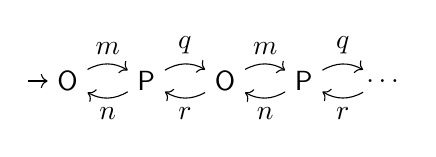
\begin{tikzpicture}[baseline=(O1.base)]
    \node (O1) at (0,0) {\kw{O}};
    \node (P1) at (1,0) {\kw{P}};
    \node (O2) at (2,0) {\kw{O}};
    \node (P2) at (3,0) {\kw{P}};
    \node (O3) at (4,0) {$\ldots$};
    \path [->] (-0.5,0) edge (O1);
    \path [->] (O1) edge[bend left] node[auto] {$m$} (P1);
    \path [->] (P1) edge[bend left] node[auto] {$n$} (O1);
    \path [->] (P1) edge[bend left] node[auto] {$q$} (O2);
    \path [->] (O2) edge[bend left] node[auto] {$r$} (P1);
    \path [->] (O2) edge[bend left] node[auto] {$m$} (P2);
    \path [->] (P2) edge[bend left] node[auto] {$n$} (O2);
    \path [->] (P2) edge[bend left] node[auto] {$q$} (O3);
    \path [->] (O3) edge[bend left] node[auto] {$r$} (P2);
  \end{tikzpicture}
  \quad
  \begin{array}{c@{\,}l@{\quad}c@{\,}l}
    m &\in M_B^\kw{Q} & q &\in M_A^\kw{Q} \\[1ex]
    n &\in M_B^\kw{A} & r &\in M_A^\kw{A}
  \end{array}
\]
The first move is always a question $m$ played by $\kw{O}$ in $B$.
The player $\kw{P}$ can conclude the current instance of $B$
with an answer $n$, or
initiate an instance of $A$
with a question $q$.
Then $\kw{O}$ can initiate a new instance of $B$
with another $m$, or
conclude any current instance of $A$
with an answer $r$.
This process goes on indefinitely.

%}}}

\subsection{Innocent strategies} %{{{

Readers familiar with traditional work on HON games \cite{something}
will recognize this description
as the \emph{well-bracketed} plays for the game ${!}A \multimap {!}B$
whose arena can be given schematically as:
\[
  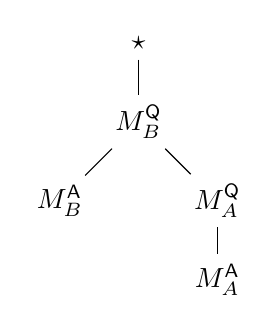
\begin{tikzpicture}
    \node (S) at (0,3) {$\star$};
    \node (BQ) at (0,2) {$M_B^\kw{Q}$};
    \node (BA) at (-1,1) {$M_B^\kw{A}$};
    \node (AQ) at (+1,1) {$M_A^\kw{Q}$};
    \node (AA) at (+1,0) {$M_A^\kw{A}$};
    \path (S) edge (BQ);
    \path (BQ) edge (BA);
    \path (BQ) edge (AQ);
    \path (AQ) edge (AA);
  \end{tikzpicture}
\]
Drawing from this work,
we can further distinguish \emph{innocent} strategies,
which handle all incoming questions $m \in M_B^\kw{Q}$
independently of the computation's history,
and therefore can be described in a particularly simple way.







%}}}

%}}}

\section{Refinement-based game semantics for C} %{{{

In this section we will give a quick overview of CompCertO
and explain how to use it in the context of our strategy model.

\subsection{Semantics of transition systems} %{{{

We now interpret the transition systems defined in \S\ref{sec:compcert}
in terms of the strategy model we have defined.
We consider a transition system $L : E \rightarrow F$
with the components $L = \langle S, {\rightarrow}, I, X, Y, F \rangle$.

In CompCert transition systems,
multiple transitions from a given state $s$
denotes demonic nondeterminism.
However,
the lack of any transition is interpreted as ``going wrong'',
in other words it denotes an undefined behavior.
To account for this idiom,
we define the notion of discontinuous choice among
a set $S \subseteq \mathcal{I}_E(A)$ of interactive computations:
\[
    \bigoplus S :=
    \begin{cases}
      \bot & \mbox{if } S = \varnothing \\
      \bigsqcap S & \mbox{otherwise}
    \end{cases}
\]
With this,
we can define the immediate behavior of a state $s \in S$ as
using the function $\delta : S \rightarrow \mathcal{I}_E(S)$
defined as:
\[
  \delta(s) :=
    \{ \kw{safe}(s) \} ;
    \left( \bigsqcap_{s \rightarrow s'} \eta(s') \right)
    \sqcap
    \left( \bigsqcap_{m \in X(s)} n \leftarrow \mathbf{I}(m) ;
            \bigoplus_{s' \in Y(s, n)} \eta(s') \right)
\]
The initial assertion ensures that unsafe states go wrong.
The subsequent demonic choice
collects transitions to other states,
either direct or after an interaction.
By iterating $\delta$, we can then compute the overall behavior of $L$:
\[
   \llbracket L \rrbracket (q) :=
     \bigoplus_{s \in I(q)}
     \left(
     \bigsqcup_{n \in \mathbb{N}}
     s' \leftarrow \delta^n(s) ; \bigsqcap_{r \in F(s')} \eta(r)
     \right)
\]

%}}}

\subsection{Simulation conventions} %{{{

Consider a simulation convention $\mathbb{R} : E_1 \Leftrightarrow E_2$
with the components $\mathbb{R} = \langle W, R^\kw{Q}, R^\kw{A} \rangle$.
We will define two adjoint strategies
which will translate questions and answers between
$E_1$ and $E_2$.
For purposes of intuition,
we can think of $E_1$ as the game $\mathcal{C}$,
$E_2$ as the game $\mathcal{A}$,
and $\mathbb{R}$ as the overall simulation convention of CompCert.

The strategy $\mathbb{R}^* : E_1 \rightarrow E_2$
is used to translate incoming calls
and is defined as follows:
\[
    \mathbb{R}^*(m_2) :=
       \bigsqcup_{m_1 \ifr{w \Vdash R^\kw{Q}} m_2}
       n_1 \leftarrow \mathbf{I}(m_1) ;
       \bigsqcap_{n_1 \ifr{w \Vdash R^\kw{A}} n_2}
       \eta(n_2)
\]
Note that the first choice ranges over the values of both
$w \in W$ and $m_1 \in M_{E_1}^\kw{Q}$,
whereas the second choice ranges only over the value of
$n_2 \in M_{E_2}^\kw{A}$.
If $m_2$ is an assembly call,
we first choose a corresponding C call $m_1$,
then pass the request along.
If there are no such calls,
the result is an undefined behavior.
When the answer $n_1$ is received,
we translate it back to an assembly return $n_2$.
The exact details of $n_2$ will be chosen by
the compiled program implementing our specification,
hence we use a demonic choice.

The strategy $\mathbb{R}_* : E_2 \rightarrow E_1$
is used to translate outgoing calls
and is defined as follows:
\[
    \mathbb{R}_*(m_1) :=
       \bigsqcap_{m_1 \ifr{w \Vdash R^\kw{Q}} m_2}
       n_2 \leftarrow \mathbf{I}(m_2) ;
       \bigsqcup_{n_1 \ifr{w \Vdash R^\kw{A}} n_2}
       \eta(n_1)
\]
Here,
the compiled system will determine
the details of the assembly call,
whereas its environment will determine
the exact assembly state returned.
Hence, the polarity of choices is reversed.

With these definitions,
given two simulation conventions
$\mathbb{R} : E_1 \Leftrightarrow E_2$ and
$\mathbb{S} : F_1 \Leftrightarrow F_2$,
we can give the concretization of a strategy
$\sigma \in \llbracket E_1 \rightarrow F_1 \rrbracket$
according to the simulation convention
$\mathbb{R} \rightarrow \mathbb{S}$
as the strategy
$\gamma_{\mathbb{R} \rightarrow \mathbb{S}}(\sigma) \in
  \llbracket E_2 \rightarrow F_2 \rrbracket$
defined by:
\[
    \gamma_{\mathbb{R} \rightarrow \mathbb{S}}(\sigma) :=
    \mathbb{R}^* \circ \sigma \circ \mathbb{S}_* \,.
\]

%}}}

\subsection{Soundness of simulations} %{{{

Putting these ingredients together,
backward simulations can be embedded as refinement:
\[
    \AxiomC{$L_1 \ge_{\mathbb{R} \rightarrow \mathbb{S}} L_2$}
    \UnaryInfC{$\gamma_{\mathbb{R} \rightarrow \mathbb{S}}
                (\llbracket L_1 \rrbracket) \sqsubseteq
                \llbracket L_2 \rrbracket$}
    \DisplayProof
\]
[Actually we could use forward sim directly,
interpreting all CompCert nondet as angelic,
which doesn't matter if we've shown they're determinate
and makes the embedding simpler.]

%}}}

\subsection{Compiler correctness} %{{{

Formulated in our setting as:
\[
    \gamma_{\mathbb{C} \twoheadrightarrow \mathbb{C}}
          (\llbracket \kw{Clight}(p) \rrbracket) \sqsubseteq
    \llbracket \kw{Asm}(p') \rrbracket
\]

%}}}

%}}}

\section{Certified abstraction layers} %{{{

\subsection{Defining layer specifications} %{{{

To define certified abstraction layers,
we can introduce a new construction is $A[S]$,
which roughly corresponds to the \emph{state monad transformer},
and adjoins a state $s \in S$ to both the questions and answers of $A$.
We can then define a state hiding operator:
\[
    \sigma : A[S] \rightarrow B[S] \vdash
    h(\sigma, s_0) : A \rightarrow B \,.
\]
The hiding operator keeps track of an internal state
initialized to $s_0$.
For every input (a question in $B$ or an answer in $A$),
$h$ adjoins the current state before passing it to $\sigma$.
For every output (an question in $A[S]$ or an answer in $B[S]$),
$h$ updates the current state with the one provided
before passing the remainder to the environment.

A $\mathcal{C}$ \emph{layer interface} is defined as
$L := \langle S, s_0, I, \sigma \rangle$,
where $S$ is the type of abstract states,
$s_0 \in S$ the initial abstract state,
$I \subseteq S$ an invariant and
$\sigma \in
 \gcat[\mathcal{C}\langle D \rangle, \mathcal{C}\langle D \rangle]$
gives the layer's specification.



Now we can use 
This allows us to define stateful strategies
using $S$ as 
using the convenience interaction monad:
$\sigma \in \gcat^i[A, B \langle S \rangle]$
to $\sigma^\dagger \in \gcat[A, B \langle S \rangle]$
to $h(\sigma^\dagger, s_0) \in \gcat[A, B]$.

%}}}

\subsection{Abstraction relations} %{{{

From the usual match/relate relations
we can formulate a Galois connexion
similar to what happens with simulation conventions
(in fact we could probably define an actual simulation convention).
Then the goal is to show that for 

%}}}

%}}}





\newpage
\appendix
\section*{Stuff from before, to redistribute}

\section{Refinement-Based Game Semantics} \label{sec:gamesem} %{{{

Our changes to the semantic framework of CompCert
and its correctness proof
ensure that they characterize the behavior of open modules,
making it possible to use them in their full generality
in the construction of larger certified systems.
To leverage this,
we must connect it to a high-level composition infrastructure.

In the following,
we present a game semantics equipped with a notion of refinement,
and which features both angelic and demonic nondeterminism.
This framework is based on an \emph{interaction monad} $\mathcal{I}_E$
modelling computations which can interact with their environment
according to the elementary game $E$.
We use this monad to build our strategy model for the
arrow games $E \rightarrow F$,
and show how to interpret the operational semantics
and simulation conventions defined in \S\ref{sec:compcert}.
We conclude by defining a notion of \emph{semantic linking}
similar to the one used in Compositional CompCert.

\subsection{The Interaction Monad} \label{sec:monad:def} %{{{

First,
we define the monad $\mathcal{I}_E(A)$
at the heart of our game semantics.
To this end,
we first define the sets of plays $P_A(V)$
for the elementary game $A$ with return values in $V$.
Plays already constitute a monad,
however we emulate the approach taken in \cite{cspdnd}
and take their \emph{completely distributive lattice completion}
to obtain a strategy domain featuring dual nondeterminism.

When $\kw{P}$ is to play,
it can either terminate with a return value $v \in A$,
or make a move $m \in M_E^\kw{P}$ and pass control to $\kw{O}$,
which is then free to resume the computation with
a move $n \in M_E^\kw{O}$ of its own,
or to abandon the computation.
Accordingly,
the plays $s \in P_E(A)$
for an elementary game $E$ and a return type $A$
are defined inductively as:
\[
  s \in P_E(A) ::= v \mid \underline{m} \mid \underline{m} ns \,,
\]
where $v \in A$, $m \in M_E^\kw{P}$ and $n \in M_E^\kw{O}$.
The prefix ordering
${\sqsubseteq} \subseteq P_E(A) \times P_E(A)$
is a natural refinement relation on plays,
and can be defined
as the smallest relation satisfying:
\[
  v \sqsubseteq v \,, \qquad
  \underline{m} \sqsubseteq \underline{m} \,, \qquad
  \underline{m} \sqsubseteq \underline{m}t \,, \qquad
  \AxiomC{$s \sqsubseteq t$}
  \UnaryInfC{$\underline{m}s \sqsubseteq \underline{m}t$}
  \DisplayProof \,.
\]

With refinement in mind,
the traditional construction of strategies
as prefix-closed sets of plays
can be understood as a lattice completion of the poset
$\langle P_E(A), {\sqsubseteq} \rangle$,
augmenting plays with angelic nondeterminism:
the behavior of a component is characterized completely
by having an angel range over all possible behaviors of the environment
and collecting the resulting plays in a set.
Prefix closure is a natural restriction because,
if $s \sqsubseteq t$ and the play $t$ is a possible outcome,
then the environment may also have stopped earlier,
resulting in the outcome $s$ instead.
Writing:
\[
  \mathcal{D}(A, {\le}) :=
    \langle
    \{ S \in \mathcal{P}(A) \mid
        \forall x, y \in A \,.\,
           x \le y \wedge y \in S \Rightarrow x \in S \},
    {\subseteq}
    \rangle
\]
for the set of down-closed subsets of $\langle A, {\le} \rangle$
ordered by inclusion,
this traditional construction can be given as
$\mathcal{S}_E(A) :=
\langle \mathcal{D}(P_E(A), {\sqsubseteq}), {\subseteq} \rangle$.

Note that this point of view suggests a new interpretation
of the determinism requirement usually placed on strategies
mentioned in \S\ref{sec:mainideas:gs:strat}.
Consider
two plays $s\underline{m_1}$ and $s\underline{m_2}$
differing only in the recorded behavior of the system
($m_1 \neq m_2$).
It is tempting to assume that
a strategy containing both of them
denotes the behavior of a non-deterministic system.
However,
under our interpretation,
while the difference between $s\underline{m_1}$ and $s\underline{m_2}$
manifests itself as the obervation of different system behaviors,
these differences are still the result of \emph{angelic} choices,
in other words they are the result of hidden choices made by the
environment.

In the model we have considered so far,
the system itself is always deterministic.
By excluding plays which differ only in their system component,
we have not enforced the determinism of the system,
but rather the \emph{determinacy} of the environment,
in the sense that angelic choices should always be observable
as distinct \kw{O}-moves.
Consequently,
an appropriate model of nondeterministic systems
cannot be obtained simply by relaxing this requirement,
and indeed in \cite{gsnondet} this approach
prevents the modelling of unbounded nondeterminism.

Instead,
we adapt the approach used in \cite{typesdnd}
and use the \emph{free completely distributive lattice}
over $\langle P_E(A), {\sqsubseteq} \rangle$
to endow strategies with both angelic and demonic nondeterminism.
Writing:
\[
  \mathcal{U}(A, {\le}) :=
    \langle
    \{ S \in \mathcal{P}(A) \mid
        \forall x, y \in A \,.\,
           x \le y \wedge x \in S \Rightarrow y \in S \},
    {\supseteq}
    \rangle
\]
for the set of up-closed subsets of $\langle A, {\le} \rangle$
ordered by containement,
the free completely distributive lattice over a poset
can be defined as the composition
$\mathcal{U}(\mathcal{D}(A, {\le}), {\subseteq})$.
We define our interaction monad as follows.

\begin{definition}
The \emph{interaction monad}
for an elementary game $E$
maps the type $A$ to the type of \emph{interactive behaviors}
$\mathcal{I}_E(A)$ where:
\[
  \langle \mathcal{I}_E(A), {\sqsubseteq} \rangle :=
    \mathcal{U}(\mathcal{S}_E(A)) \,.
\]
\end{definition}

In this construction,
the \emph{inner} sets $S \in \mathcal{S}_E(A)$
are similar to traditional strategies and
can be interpreted in the usual way,
noting however that their consistuent plays
are the result of angelic choices
no matter how and when these choices become observable.
The \emph{outer} set records \emph{demonic} choices,
and can be interpreted as follows:
the presence in the outer set $x \in \mathcal{I}_E(A)$
of an inner set $S \in x$
indicates that the demon has a strategy
to ensure that the outcome remains in $S$
no matter what the angel does.
It is natural for $x$ to be up-closed:
if $S \subseteq T$ and the demon can make sure
the outcome is contained in $S$,
then the outcome will be contained in $T$ as well.

\subsection{Operations}

\subsubsection{Termination}

The unit $\eta^E_A : A \rightarrow \mathcal{I}_E(A)$
of the interaction monad
assigns to a value $v \in A$ the computation
which simply returns $v$ immediately.
Because the environment is never in control,
the system can ensure that the outcome is always
the terminated play $v$.
In other words,
the demon has a strategy to ensure that the outcome is in $S$
whenever $v \in S$:
\[
  \eta^E_A(v) :=
    \{ S \in \mathcal{D}(P_E(A), {\sqsubseteq}) \mid v \in S \} \,.
\]

\subsubsection{Nondeterminism}

The refinement lattice over $\mathcal{I}_E(A)$
provides unbounded demonic choices
in the form of arbitrary meets
(realized as the union of the outer sets),
and unbounded angelic choices
in the form of arbitrary joins
(realized as the intersection of the outer sets).
A refinement $x \sqsubseteq y$ expresses that
$y$ offers fewer demonic choices and more angelic choices than $x$.

In particular,
the least element $\bot = \bigsqcup \varnothing$
corresponds to a situation where the environment has no choices
and the computation cannot be resumed.
It can be refined by any other computation and
we will use it to interpret undefined behaviors and silent divergence.
Conversely,
the greatest element $\top = \bigsqcap \varnothing$
corresponds to the \emph{magic} behavior
which refines all others:
the system has no choices,
therefore any behavior is vacuously satisfactory.

Another special case of angelic choice is
the \emph{assertion} of a proposition $P$,
which returns the trivial value $*$ if $P$ holds
and is equal to $\bot$ otherwise:
\[ \{P\} \in \mathcal{I}_E(\{*\}) :=
    \bigsqcup \{ \eta(*) \mid P \} \]
Dually,
the \emph{assumption} of $P$
is defined as follows,
and is equal to $\top$ when $P$ does not hold:
\[ [P] \in \mathcal{I}_E(\{*\}) :=
    \bigsqcap \{ \eta(*) \mid P \} \]

\subsubsection{Conventions}

Because the lattice completion is itself a monad,
many operations on interactive computations
can be defined by specifying their action on plays.
Individual plays $s \in P_E(A)$ can be monotonically promoted to
interactive computations by the completion's unit as:
\[
    {\uparrow \downarrow}(s) =
      \{ S \in \mathcal{S}_E(A) \mid s \in S \}
\]
Furthermore,
an monotonic operator $f : P_E(A) \rightarrow \mathcal{I}_E(B)$
defined on plays can be extended to computations.
For $x \in \mathcal{I}_E(A)$, we will write:
\[
  f(x) := \bigsqcap_{S \in x} \bigsqcup_{s \in S} f(s)
\]
When the result is unambiguous we will use both constructions
implicitely.
Note that the promoted operators
distribute over arbitrary unions and intersections, so that
$f(\bigsqcap X) = \bigsqcap_{x \in X} f(x)$ and
$f(\bigsqcup X) = \bigsqcup_{x \in X} f(x)$.
This means proofs involving operators defined on plays
can often themselves be carried out at the level of plays.

\subsubsection{Sequential composition}

We start by defining the interaction monad's Kleisli extension
of a continuation $f : A \rightarrow \mathcal{I}_E(B)$
as an operator on traces
$f^\dagger : P_E(A) \rightarrow \mathcal{I}_E(B)$:
\[
  f^\dagger(v) := f(v) \qquad
  f^\dagger(\underline{m}) := \underline{m} \qquad
  f^\dagger(\underline{m} n s) :=
    \underline{m} \sqcup \underline{m} n f^\dagger(s) \,.
\]
The lattice completion is first used in the recursive case above
to apply the function $t \mapsto \underline{m} n t$
to the computation $f^\dagger(s)$,
then used to extend $f^\dagger$ as a whole to the desired
$f^\dagger : \mathcal{I}_E(A) \rightarrow \mathcal{I}_E(B)$.
Following usual conventions, we will use the notations:
\begin{align*}
  v \leftarrow x ; M &:= (v \mapsto M)^\dagger(x) \\
  x ; M &:= ({-} \mapsto M)^\dagger(x)
\end{align*}

\subsubsection{Interaction}

Another elementary operation
is the interaction primitive
$\mathbf{I}_E : M_E^\kw{Q} \rightarrow \mathcal{I}_E(M_E^\kw{A})$.
The computation $\mathbf{I}_E(m)$
asks the question $m \in M_E^\kw{Q}$ to the environment
and returns the corresponding answer.
It can be defined as:
\[
    \mathbf{I}_E(m) := \underline{m} n n 
\]
Note that in the play $\underline{m} n n$,
the first occurence of $n$ is the environment's answer,
whereas the second occurence is the value returns by $\mathbf{I}_E(m)$.

\subsubsection{Interactive substitution}

The interactions of a computation $x \in \mathcal{I}_E(A)$
can be interpreted in terms of another elementary game
by substituting for each one a behavior specified by
the Kleisli morphism
$f : M_E^\kw{Q} \rightarrow \mathcal{I}_F(M_E^\kw{A})$.
The result is a computation $x[f] \in \mathcal{I}_F(A)$,
which can be defined in terms of traces as follows:
\[
  v[f] := v \qquad
  \underline{m}[f] := f(m) ; \bot \qquad
  \underline{m}ns[f] := r \leftarrow f(m) ; \{r = n\} ; s[f]
\]
Note that $\mathbf{I}(m)[f] = f(m)$,
$x[\mathbf{I}] = x$,
and $x[m \mapsto f(m)[g]] = x[f][g]$.

%}}}

\subsection{Game semantics}

The interaction monad
models the behavior of
nondeterministic interactive computations
which can interact with their environment
according to an elementary game $E$.
We now use this infrastructure
to define our game semantics.

Innocent strategies for the game $E \rightarrow F$
can be represented using Kleisli morphisms of
the interaction monad:
\[
  \llbracket E \rightarrow F \rrbracket :=
  M_F^\kw{Q} \rightarrow \mathcal{I}_E(M_F^\kw{A}) \,.
\]
Given a question $q \in M_F^\kw{Q}$ for the game $F$,
a strategy $\sigma \in \llbracket E \rightarrow F \rrbracket$
can interact with the environment
indefinitely by asking questions of $E$,
and can eventually terminate by producing an answer $r \in M_F^\kw{A}$.

In the following,
after establishing the categorical structure
of this game semantics,
we show how
the operational semantics
and simulation conventions
defined for CompCert in \S\ref{sec:compcert}
can be interpreted in this framework.
We then define a notion of \emph{horizontal composition}
which mirrors the semantic linking operator
of Compositional CompCert.

\subsubsection{Composition of strategies}

Given the strategies
$\sigma \in \llbracket F \rightarrow G \rrbracket$ and
$\tau \in \llbracket E \rightarrow F \rrbracket$,
their composition
$\sigma \circ \tau \in \llbracket E \rightarrow G \rrbracket$
can be defined as a special case of interactive substitution:
\[
    \sigma \circ \tau := q \mapsto \sigma(q)[\tau]
\]
The interaction primitive
$\mathbf{I}_E \in \llbracket E \rightarrow E \rrbracket$
plays the role of the identity strategy.

\subsection*{[Sections integrated]}

\subsection{Multi-module programs}

Ultimately,
the compilation units translated by CompCert
are converted to machine code
and combined by a linker into a single
binary image.
Following Compositional CompCert,
we model this process by defining a notion of
\emph{semantic linking},
and using it to characterize the semantics
of programs which consist of several compilation units.

In the remainder of this section,
we consider a CompCert language $L$
with compilation units taken in the set $U$,
such that the semantics of $M \in U$
are described by the transition system $L(M) : E \rightarrow E$.
We will give a compositional semantics
for multi-module programs of the form:
\[
    p = (M_1; \cdots; M_n) \in U^* \,.
\]
We will assume that the components have disjoint domains
$D_1, \ldots, D_n \subseteq M_E^\kw{Q}$,
so that for any question $q \in M_E^\kw{Q}$
we have $\llbracket L(M_i) \rrbracket = \bot$
for all indices $i$ but one.

Relating the notion of semantic linking defined here
with the syntactic linking defined in CompCert
at the level of C and assembly programs
is left as future work.

\subsubsection{Horizontal composition}

If a component $M_1$ calls functions defined
in the component $M_2$,
the composition of strategies
can already compute their combined behavior:
\[
    \llbracket L(M_1) \rrbracket \circ
    \llbracket L(M_2) \rrbracket \,.
\]
However,
this is insufficient to account for
the potential two-way interaction between $M_1$ and $M_2$
since any external call performed by $M_2$
will be directed to the environment.
In addition,
in this configuration the environment
is unable to call the function of $M_2$ directly.
On the other hand,
the \emph{flat composition} of the behaviors:
\[
    \llbracket L(M_1) \rrbracket \sqcup
    \llbracket L(M_2) \rrbracket
\]
let the environment communicate with each component directly,
but does not let the components interact with each other.

To synthesize the two aspects,
we define the \emph{horizontal composition}
of two strategies $\sigma_1, \sigma_2 \in \llbracket E \rightarrow E \rrbracket$
with respective domains $D_1, D_2 \subseteq M_E^\kw{Q}$
as the strategy $\sigma_1 \bullet \sigma_2 : \llbracket E \rightarrow E
\rrbracket$ defined by:
\[
    \sigma_1 \bullet \sigma_2 :=
      \bigsqcup_{n \in \mathbb{N}} (\sigma_1 \sqcup \sigma_2)^n \circ
        (q \mapsto \{ q \notin D_1 \cup D_2 \} ; \mathbf{I}(q))
 \,,
\]
where $\sigma^0 = \mathbf{I}$ and $\sigma^{n+1} = \sigma^n \circ
\sigma$.

\subsubsection{Semantics of multi-module programs}

Using horizontal composition,
the semantics of the multi-module program $p$
can be expressed as:
\[
    \llbracket p \rrbracket :=
    \llbracket L(M_1) \rrbracket \bullet \cdots \bullet
    \llbracket L(M_n) \rrbracket
\]

This concludes the outline of our refinement-based game semantics.
We believe the approach presented here can be applied to a larger class
of game models and intend to investigate its applications
and properties further in future work.

%}}}








\end{document}
